%% REPLACE SXXXXXX with your student number
\def\studentNumber{S2414220}


%% START of YOUR ANSWERS
%% Add answers to the questions below, by replacing the text inside the brackets {} for \youranswer{ "Text to be replaced with your answer." }. 
%
% Do not delete the commands for adding figures and tables. Instead fill in the missing values with your experiment results, and replace the images with your own respective figures.
%
% You can generally delete the placeholder text, such as for example the text "Question Figure 2 - Replace the images ..." 
%
% There are 18 TEXT QUESTIONS (a few of the short first ones have their answers added to both the Introduction and the Abstract). Replace the text inside the brackets of the command \youranswer with your answer to the question.
%
% There are also 3 "questions" to replace some placeholder FIGURES with your own, and 3 "questions" asking you to fill in the missing entries in the TABLES provided. 
%
% NOTE! that questions are ordered by the order of appearance of their answers in the text, and not by the order you should tackle them. Specifically, you cannot answer Questions 2, 3, and 4 before concluding all of the relevant experiments and analysis. Similarly, you should fill in the TABLES and FIGURES before discussing the results presented there. 
%
% NOTE! If for some reason you do not manage to produce results for some FIGURES and TABLES, then you can get partial marks by discussing your expectations of the results in the relevant TEXT QUESTIONS (for example Question 8 makes use of Table 1 and Figure 2).
%
% Please refer to the coursework specification for more details.


%% - - - - - - - - - - - - TEXT QUESTIONS - - - - - - - - - - - - 



%% Question 1:
% \newcommand{\questionOne} {
% \youranswer{Question 1 - Explain what these figures contain and how the curves evolve, and spot where overfitting occurs. Reason based on the min/max points and velocities (direction and magnitude of change) of the accuracy and error curves}
% }

\newcommand{\questionOne} {
    \youranswer{
        Based on Figure 1, the fundamental problem identified is \textbf{overfitting}.
        \begin{itemize}
            \item \textbf{Error Curves (Fig 1a):} The training error (solid line) decreases monotonically, approaching zero, indicating the model is effectively learning the training data. However, the validation error (dashed line) decreases initially but reaches a minimum around epoch 15, after which it begins to rise significantly. This divergence indicates that while the model continues to memorize the training set, its ability to generalize to unseen data is deteriorating.
            \item \textbf{Accuracy Curves (Fig 1b):} Similarly, the training accuracy reaches near-perfect levels ($>95\%$), while the validation accuracy plateaus and slightly degrades.
        \end{itemize}
        This generalization gap suggests the model capacity is too high relative to the dataset size, leading it to learn noise rather than underlying patterns.
        }
}

%% Question 2:
\newcommand{\questionTwo} {
\youranswer{
    Figure~\ref{fig:width} and Table~\ref{tab:width_exp} present 
    the results of varying network width (32, 64, and 128 hidden units).
    
    As shown in Figure~\ref{fig:width_acccurves}, validation accuracy 
    improves from 79.0\% (32 units) to 80.5\% (64 units), with marginal 
    gains to 80.7\% for 128 units. Figure~\ref{fig:width_errorcurves} 
    reveals that while training error decreases monotonically with width, 
    validation error exhibits a U-shaped pattern, with the 64-unit network 
    achieving the lowest validation error (0.677).
    
    The 128-unit network demonstrates severe overfitting, with validation 
    error increasing to 0.975 despite achieving the lowest training error 
    (0.156), resulting in a generalization gap of 0.819.
}
}

%% Question 3:
\newcommand{\questionThree} {
\youranswer{
    The experimental results demonstrate a consistent yet non-linear 
    relationship between network width and performance, aligning well 
    with established theory on model capacity and generalization.
    
    \textbf{Consistent patterns:} Training error decreases monotonically 
    with width (0.552 → 0.343 → 0.156), confirming that wider networks 
    possess greater representational capacity. However, validation 
    performance does not follow this trend, with the 64-unit network 
    achieving the best generalization (validation error: 0.677).
    
    \textbf{Theoretical alignment:} These results exemplify the 
    bias-variance tradeoff. The 32-unit network exhibits underfitting 
    (high bias), with training and validation curves remaining close 
    but at suboptimal error levels. The 128-unit network demonstrates 
    severe overfitting (high variance), memorizing training data rather 
    than learning generalizable patterns. The 64-unit configuration 
    represents an optimal balance.
    
    \textbf{Literature context:} This phenomenon is well-documented 
    in deep learning literature, where increasing model capacity without 
    regularization eventually degrades generalization performance. 
    The diminishing returns in validation accuracy (64→128: +0.2\%) 
    despite dramatic improvements in training error (64→128: -54\%) 
    suggest that regularization techniques are necessary to leverage 
    larger network capacities effectively.
}
}

%% Question 4:
\newcommand{\questionFour} {
\youranswer{Figure~\ref{fig:depth} and Table~\ref{tab:depth_exps} present the 
results of varying network depth from 1 to 3 hidden layers. While 
validation accuracy increases modestly with depth (80.2\% → 81.6\% 
→ 82.1\%), validation error exhibits a concerning trend, escalating 
from 0.989 (1 layer) to 1.734 (3 layers) — a 75\% increase.

The 2- and 3-layer networks achieve very low training errors (~0.1) 
and high training accuracies (~96\%), yet their validation errors 
are significantly worse than the single-layer network, revealing 
severe overfitting.}
}

%% Question 5:
\newcommand{\questionFive} {
\youranswer{The results reveal a critical insight: **increased depth without 
regularization degrades generalization performance** despite marginal 
improvements in validation accuracy.

\textbf{Overfitting severity:} The generalization gap grows 
dramatically with depth: 0.825 (1 layer) → 1.445 (2 layers) → 
1.621 (3 layers). This is substantially worse than the width 
experiments (Q2-Q3), where the maximum gap was 0.819.

\textbf{Accuracy vs. Cross-Entropy Discrepancy:} The contradiction 
between rising validation accuracy and exploding validation error 
indicates that deeper models make correct predictions but with 
poorly calibrated probability estimates — a hallmark of memorization 
rather than generalization.

\textbf{Comparison to Theory:} While deeper networks theoretically 
possess greater representational power, this advantage is nullified 
by overfitting in the absence of regularization techniques. The 
results underscore that **depth is a double-edged sword**, requiring 
careful regularization (Dropout, Batch Normalization) to realize its 
benefits — motivating the regularization experiments in subsequent 
sections.}
}


%% Question 6:
\newcommand{\questionSix} {
\youranswer{
    Elastic Net regularization combines L1 and L2 penalties to leverage 
    the complementary strengths of both approaches: L1's feature selection 
    (sparsity) and L2's weight shrinkage (stability).
    
    \textbf{Combined Loss Function:}
    \begin{equation}
        \mathcal{L}_{\text{total}} = \mathcal{L}_{\text{CE}}(y, t) + 
        \lambda_1 \sum_{l=1}^{L} \|W^{(l)}\|_1 + 
        \lambda_2 \sum_{l=1}^{L} \|W^{(l)}\|_2^2
    \end{equation}
    
    where:
    \begin{itemize}
        \item $\mathcal{L}_{\text{CE}}(y, t)$ is the cross-entropy loss 
              between predictions $y$ and targets $t$
        \item $W^{(l)}$ denotes the weight matrix of layer $l$
        \item $\|W^{(l)}\|_1 = \sum_{i,j} |w_{ij}^{(l)}|$ is the L1 norm 
              (Manhattan distance)
        \item $\|W^{(l)}\|_2^2 = \sum_{i,j} (w_{ij}^{(l)})^2$ is the 
              squared L2 norm (Euclidean distance)
        \item $\lambda_1 \geq 0$ controls sparsity (higher → more zeros)
        \item $\lambda_2 \geq 0$ controls shrinkage (higher → smaller weights)
        \item $L$ is the total number of layers with learnable parameters
    \end{itemize}
    
    \textbf{Benefits:} This combination handles correlated features better 
    than L1 alone, produces sparse solutions unlike L2 alone, and provides 
    a flexible regularization spectrum by tuning $\lambda_1$ and $\lambda_2$ 
    independently.
}
}


%% Question 7:
\newcommand{\questionSeven} {
\youranswer{Question 7 - Assume you had a limited experiment budget for exactly \textbf{4} experiment runs dedicated to testing the effectiveness of your proposed combination of L1 and L2 Regularization in Section~\ref{sec:L1L2combo}. Argue for which 4 configurations to run based on any previous results or other information you consider relevant. Run those experiments and add the results in Table~4 and Figure~5 (you will then discuss those results alongside all others in the next question below).

(Even if you have not managed to implement your L1 and L2 combination; still argue based on your proposed approach).

}
}


%% Question 8:
\newcommand{\questionEight} {
\youranswer{Question 8 - Explain the experimental details (e.g. hyperparameters), discuss the results in terms of their generalisation performance and overfitting. Select and test the best performing model as part of this analysis.
}
}


%% Question 9:
\newcommand{\questionNine} {
\youranswer{Question 9 - A colleague proposed using a custom activation function (which can be identified as CustomActivationLayer() in your Coursework\_1.ipynb notebook and the mlp package). Run the prepared experiment in the "Problematic Training" cell in your Coursework\_1.ipynb notebook, and display the results in Figure~6. Analyse the results. Is the model overfitting? Explain the cause of the problematic performance of the model?
}
}




%% Question 10:
\newcommand{\questionTen} {
\youranswer{Question 10 - Briefly draw your conclusions based on the results from the previous sections (what are the take-away messages?), discussing them in the context of the overall literature, and conclude your report with a recommendation for future directions}
}

%% - - - - - - - - - - - - FIGURES - - - - - - - - - - - - 

%% Question Figure 2:
\newcommand{\questionFigureTwo} {
\youranswer{Question Figure 2 - Replace the images in Figure 2 with figures depicting the accuracy and error, training and validation curves for your experiments varying the number of hidden units.
%
\begin{figure}[t]
    \centering
    \begin{subfigure}{\linewidth}
        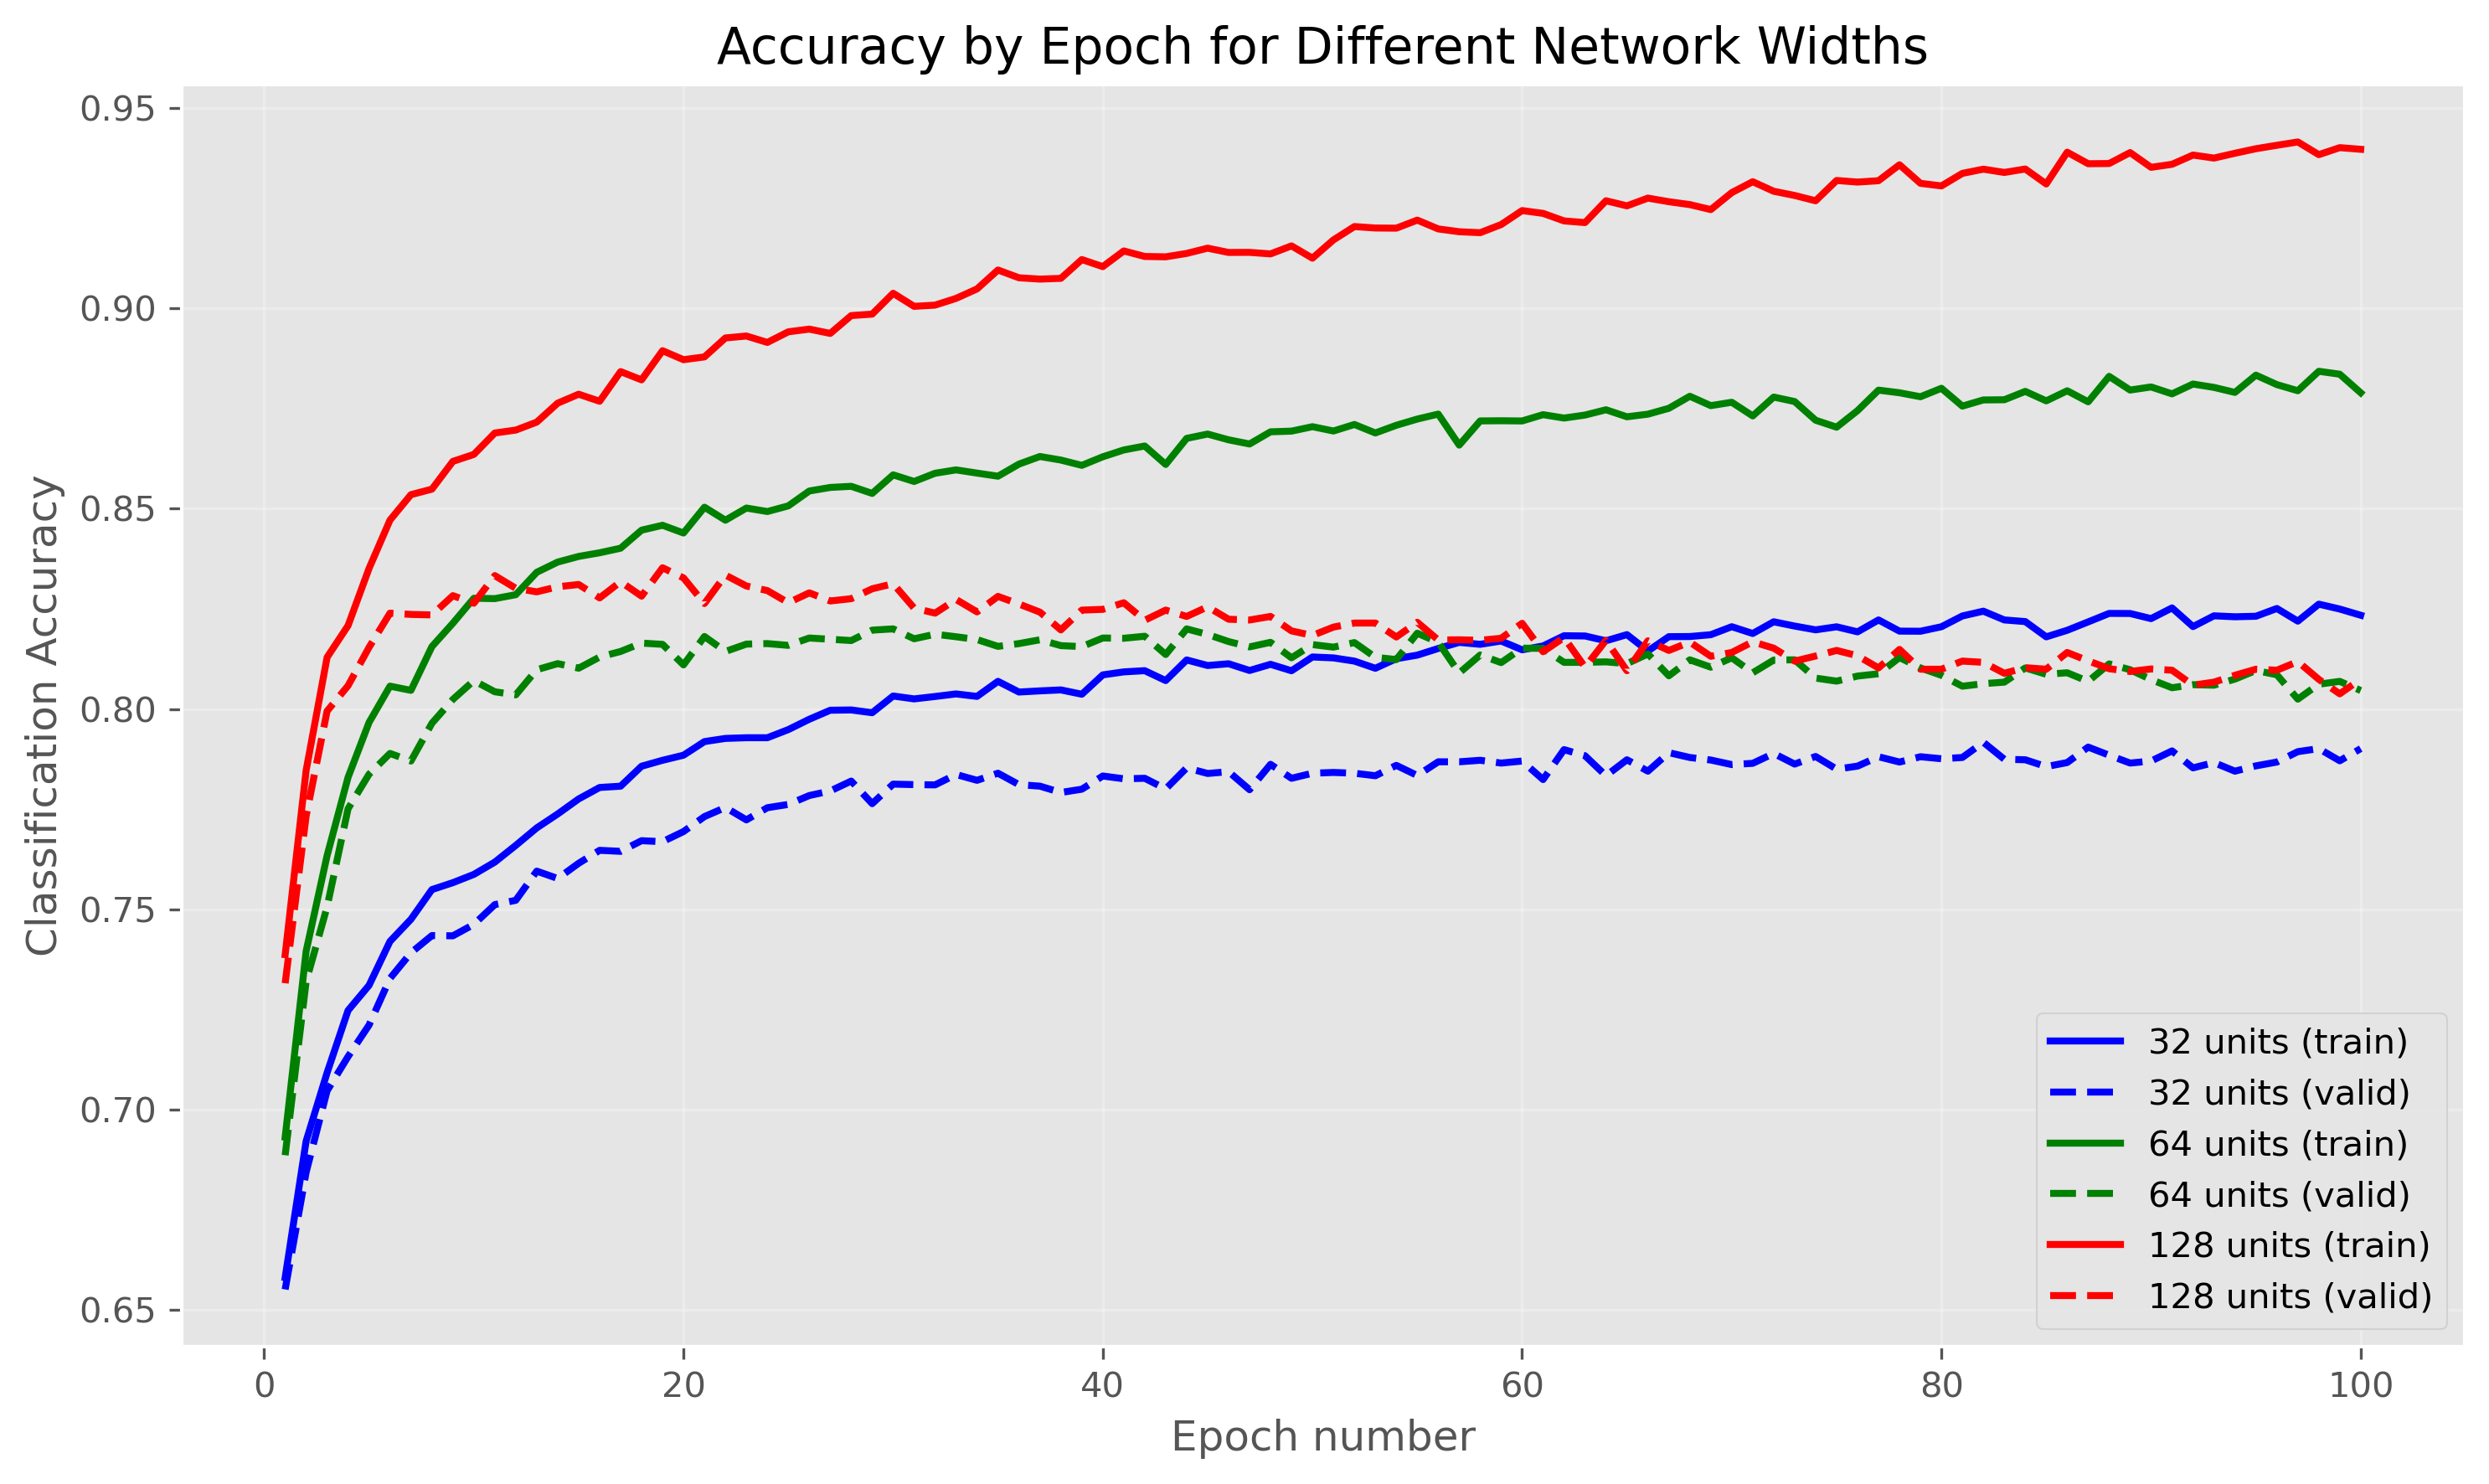
\includegraphics[width=\linewidth]{figures/empty_acc_curve_width.png}
        \caption{accuracy by epoch}
        \label{fig:width_acccurves}
    \end{subfigure} 
    \begin{subfigure}{\linewidth}
        \centering
        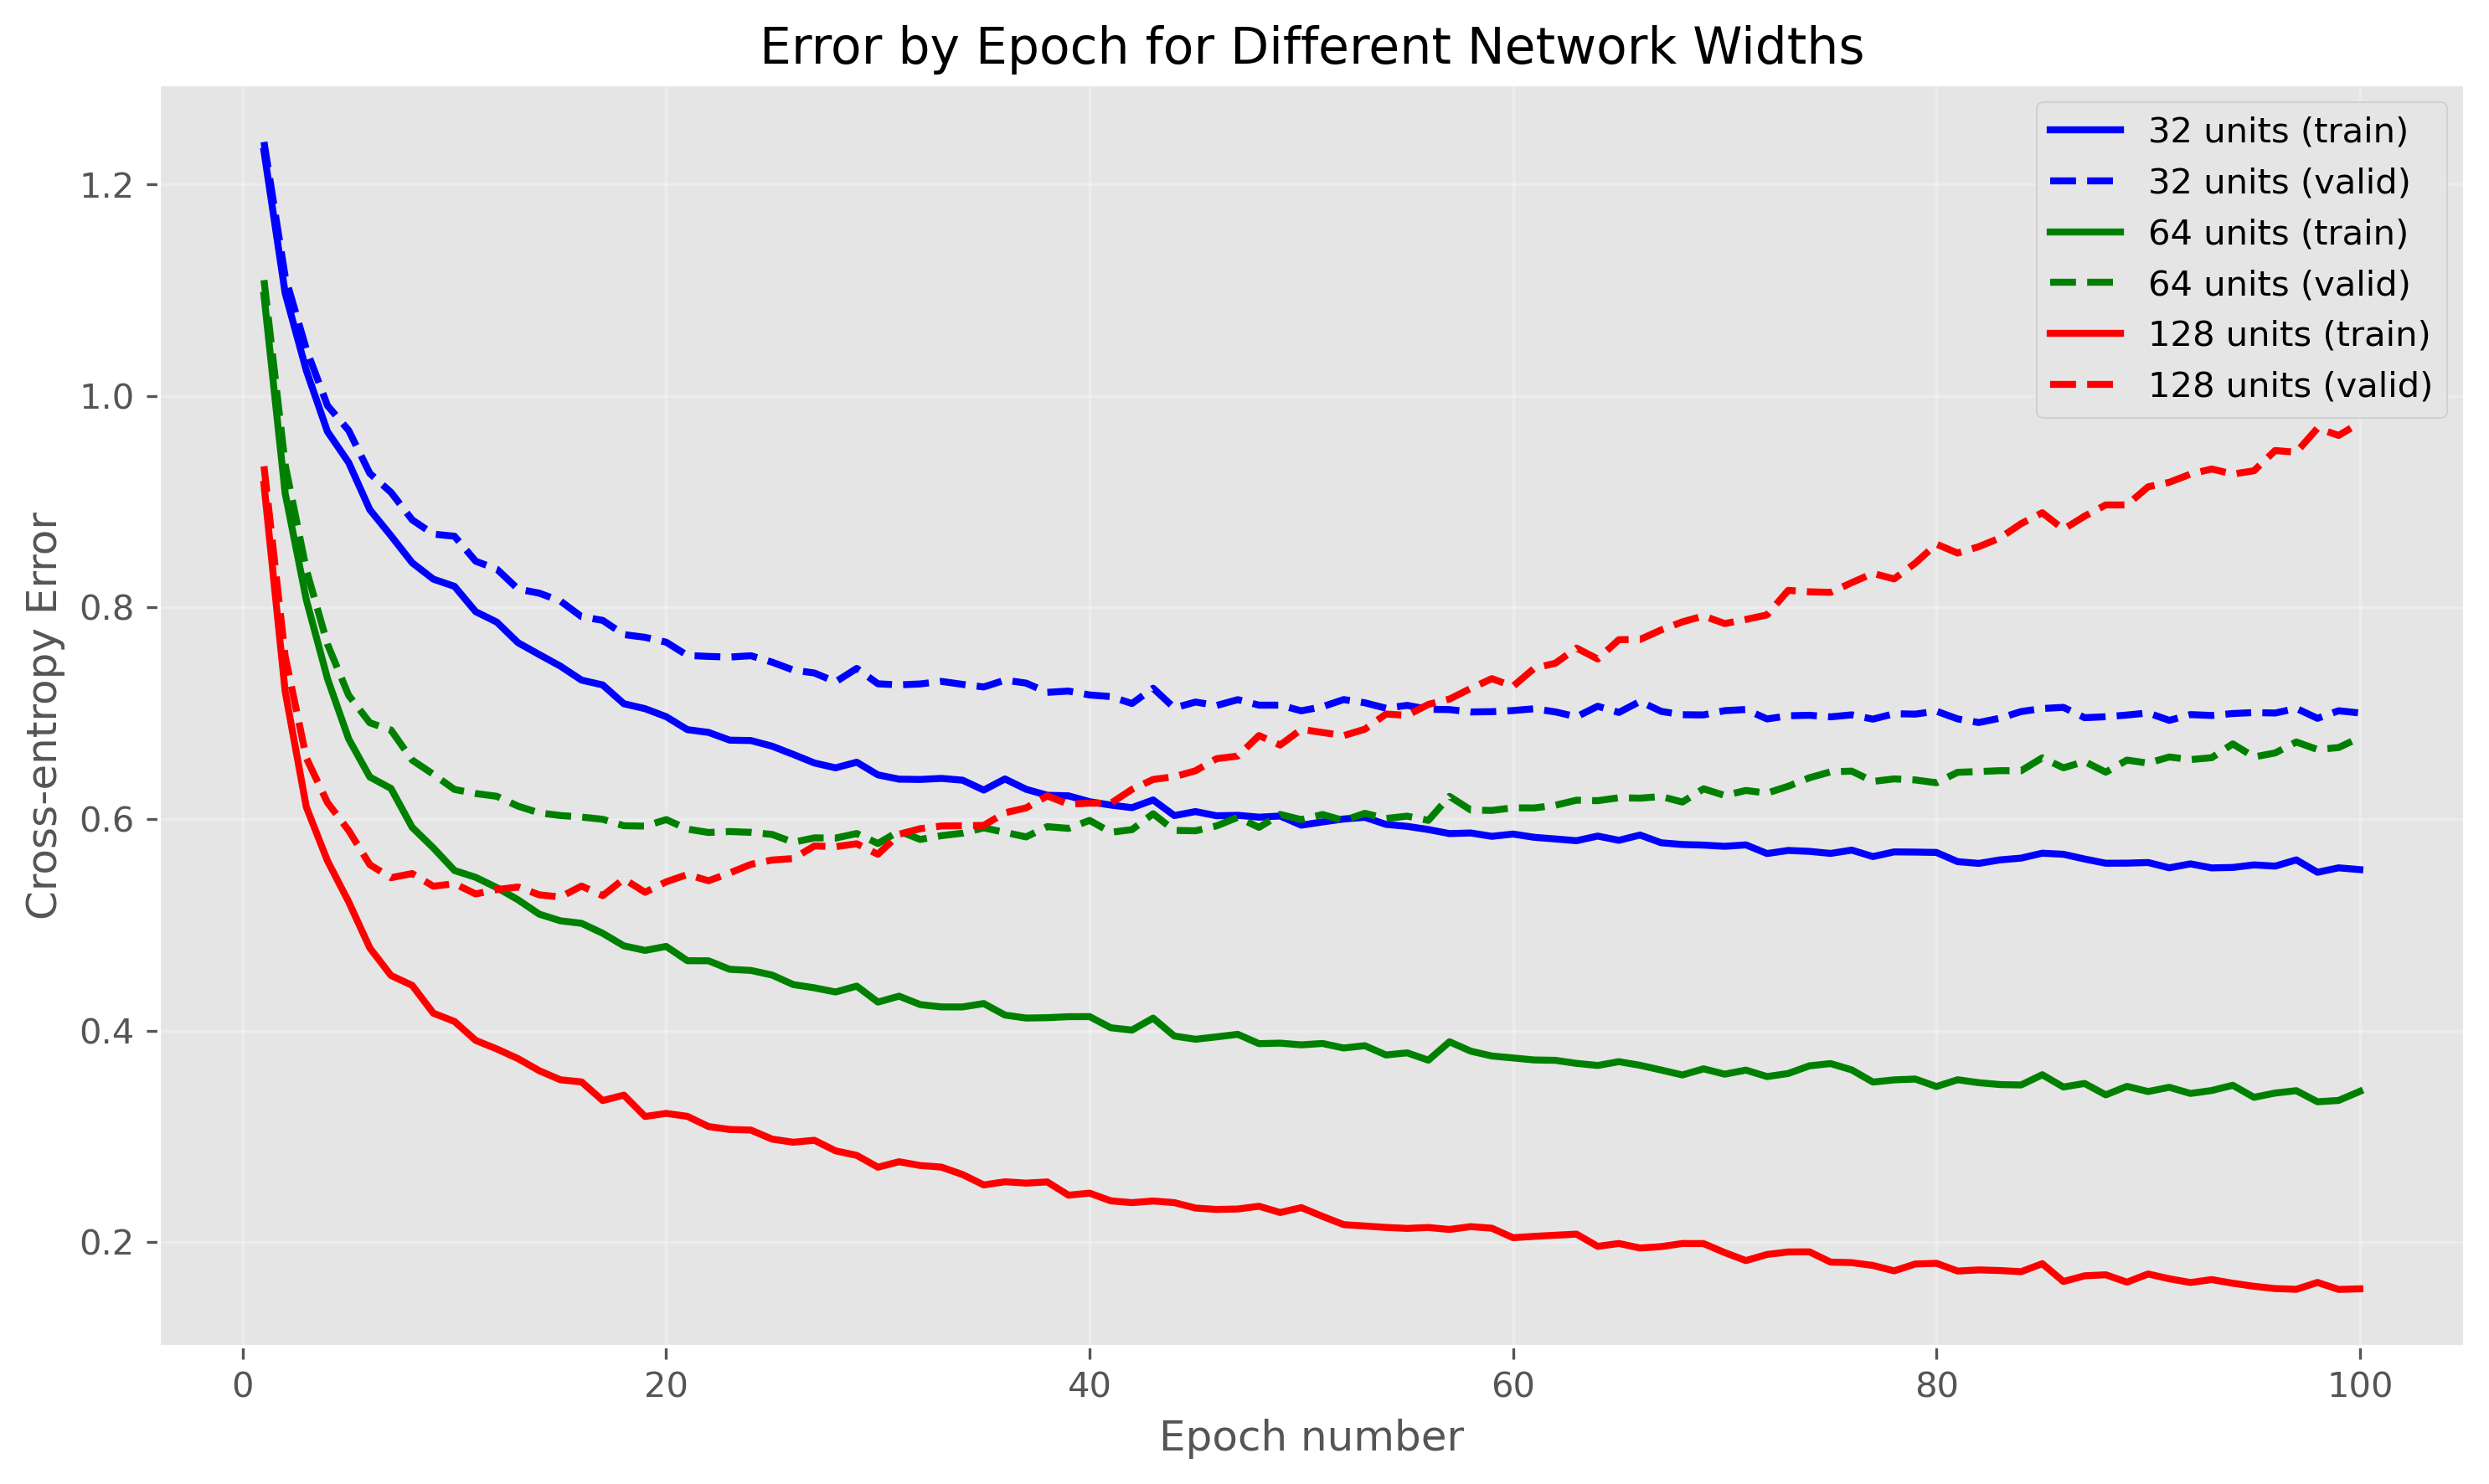
\includegraphics[width=\linewidth]{figures/empty_error_curve_width.png}
        \caption{error by epoch}
        \label{fig:width_errorcurves}
    \end{subfigure} 
    \caption{Training and validation curves in terms of classification accuracy (a) and cross-entropy error (b) on the EMNIST dataset for different network widths.}
    \label{fig:width}
\end{figure} 
}
}

%% Question Figure 3:
\newcommand{\questionFigureThree} {
\youranswer{Question Figure 3 - Replace these images with figures depicting the accuracy and error, training and validation curves for your experiments varying the number of hidden layers.
%
\begin{figure}[t]
    \centering
    \begin{subfigure}{\linewidth}
        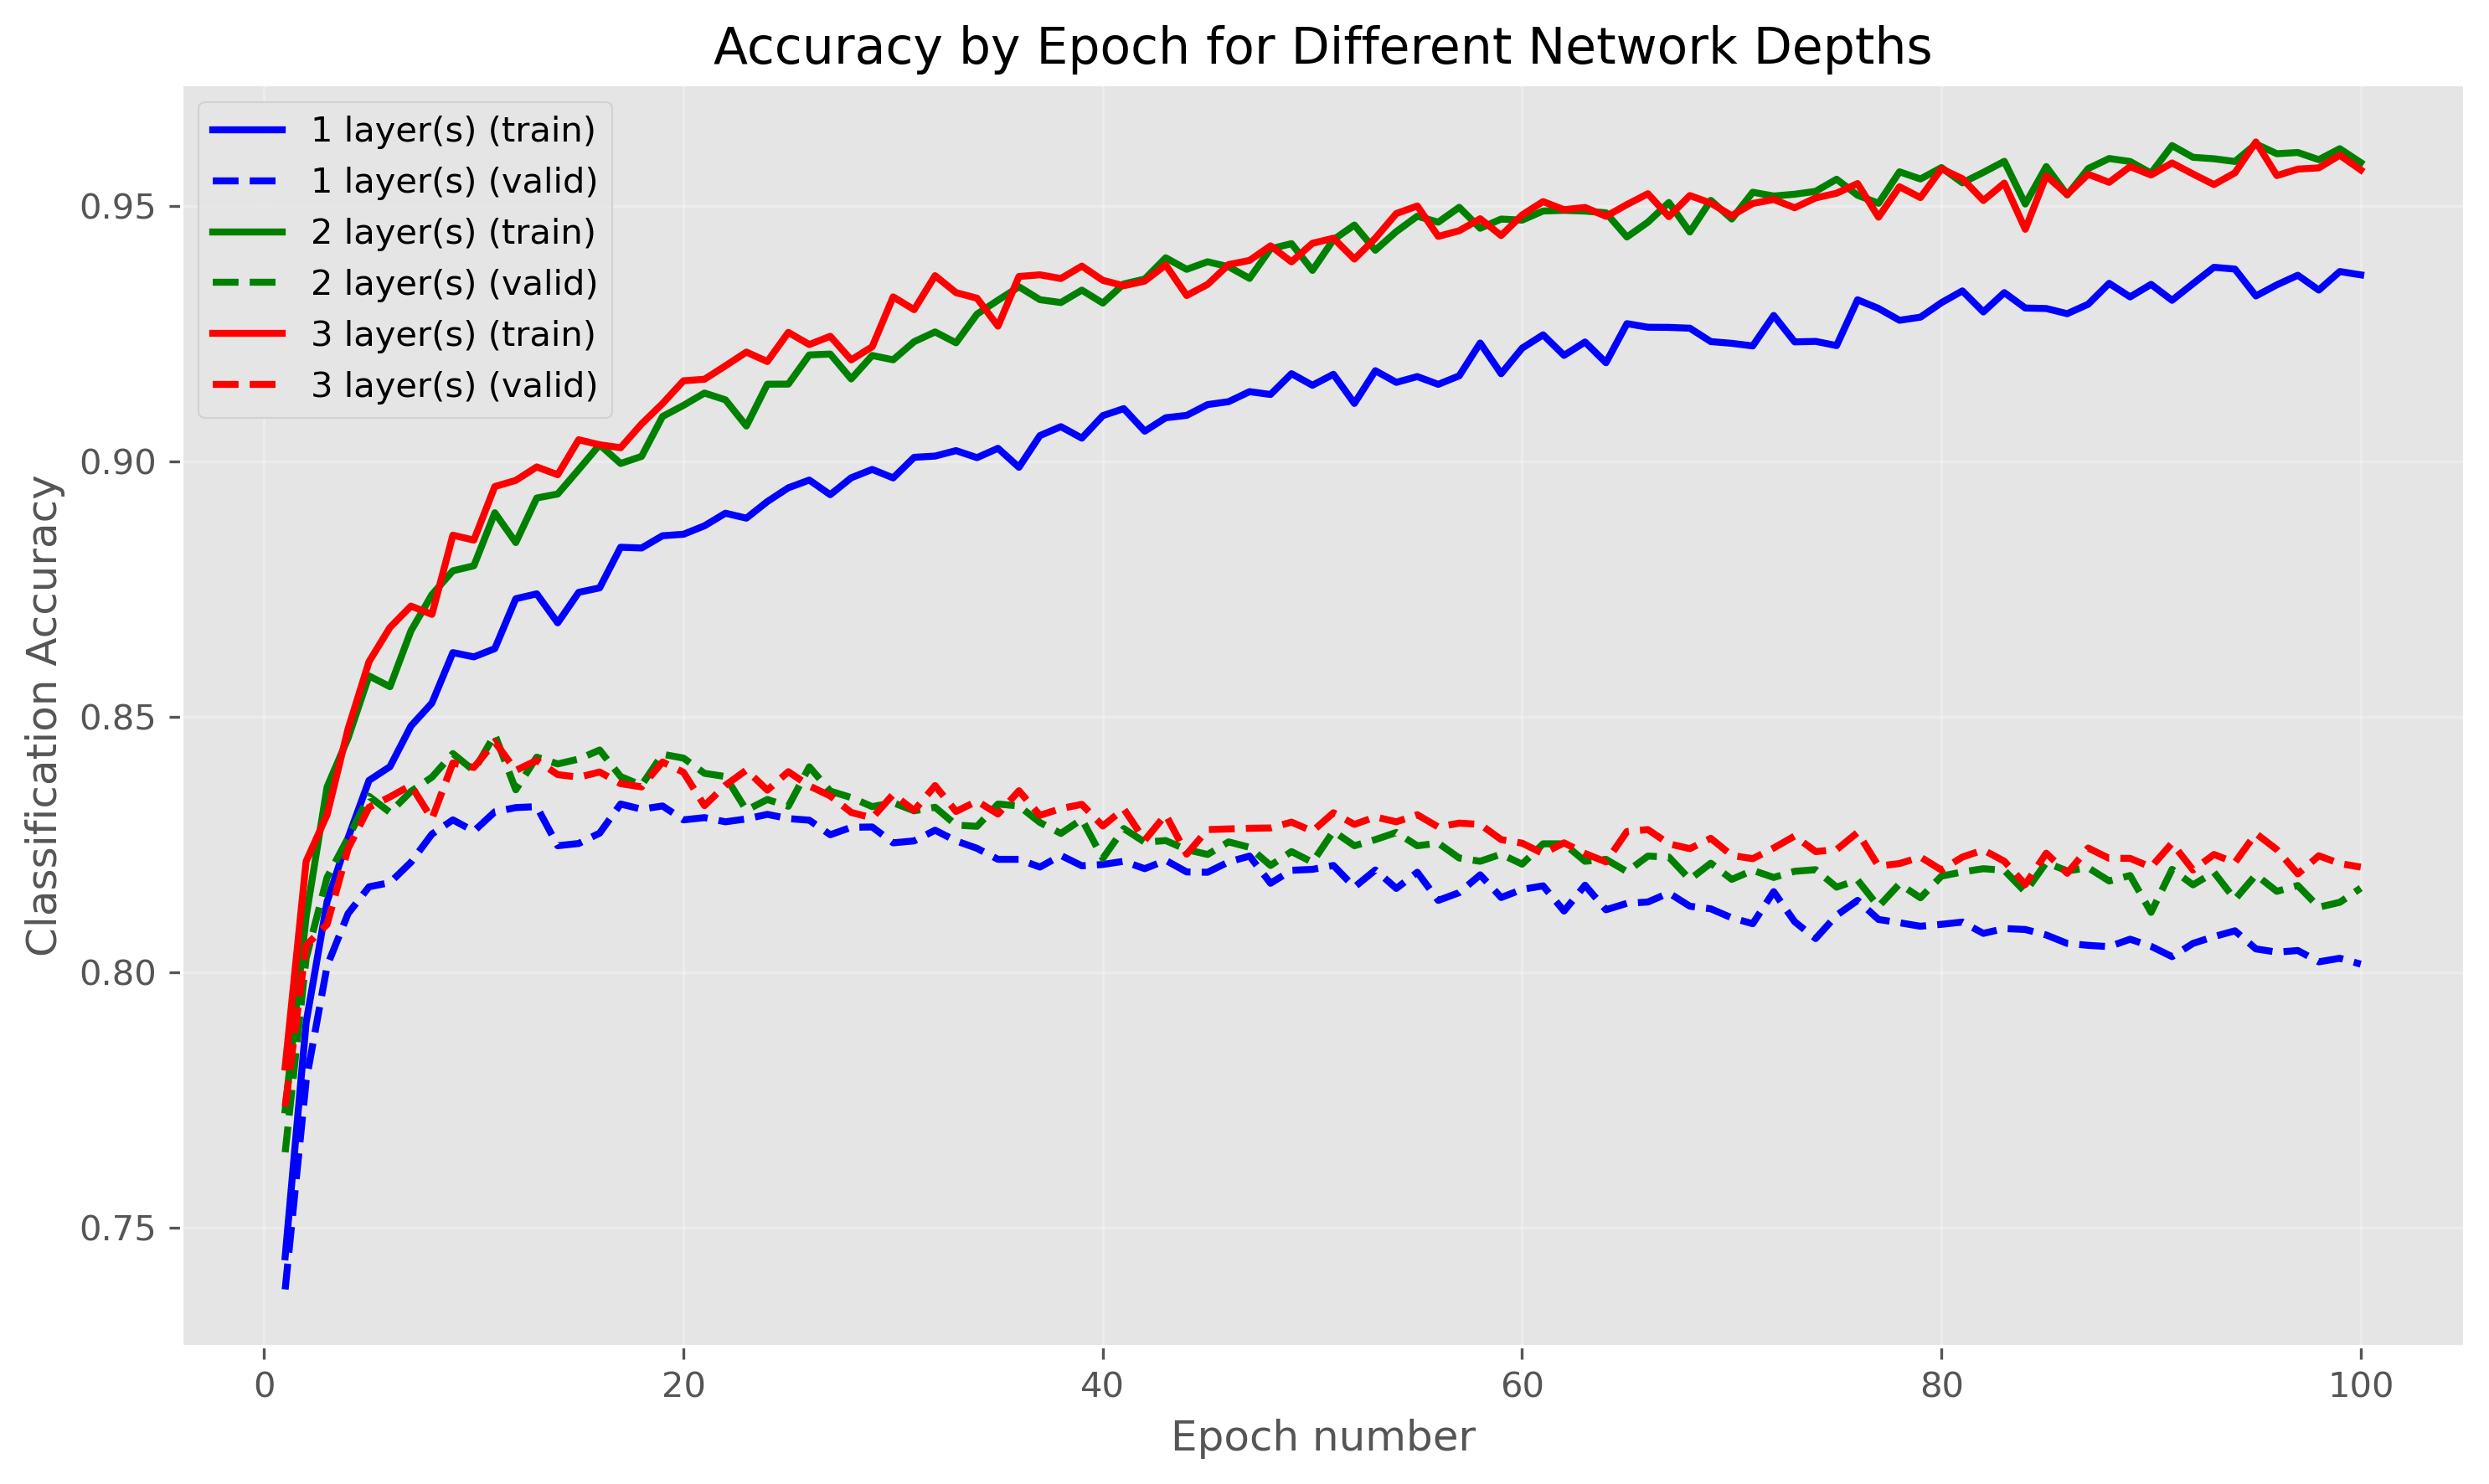
\includegraphics[width=\linewidth]{figures/empty_acc_curve_depth.png}
        \caption{accuracy by epoch}
        \label{fig:depth_acccurves}
    \end{subfigure} 
    \begin{subfigure}{\linewidth}
        \centering
        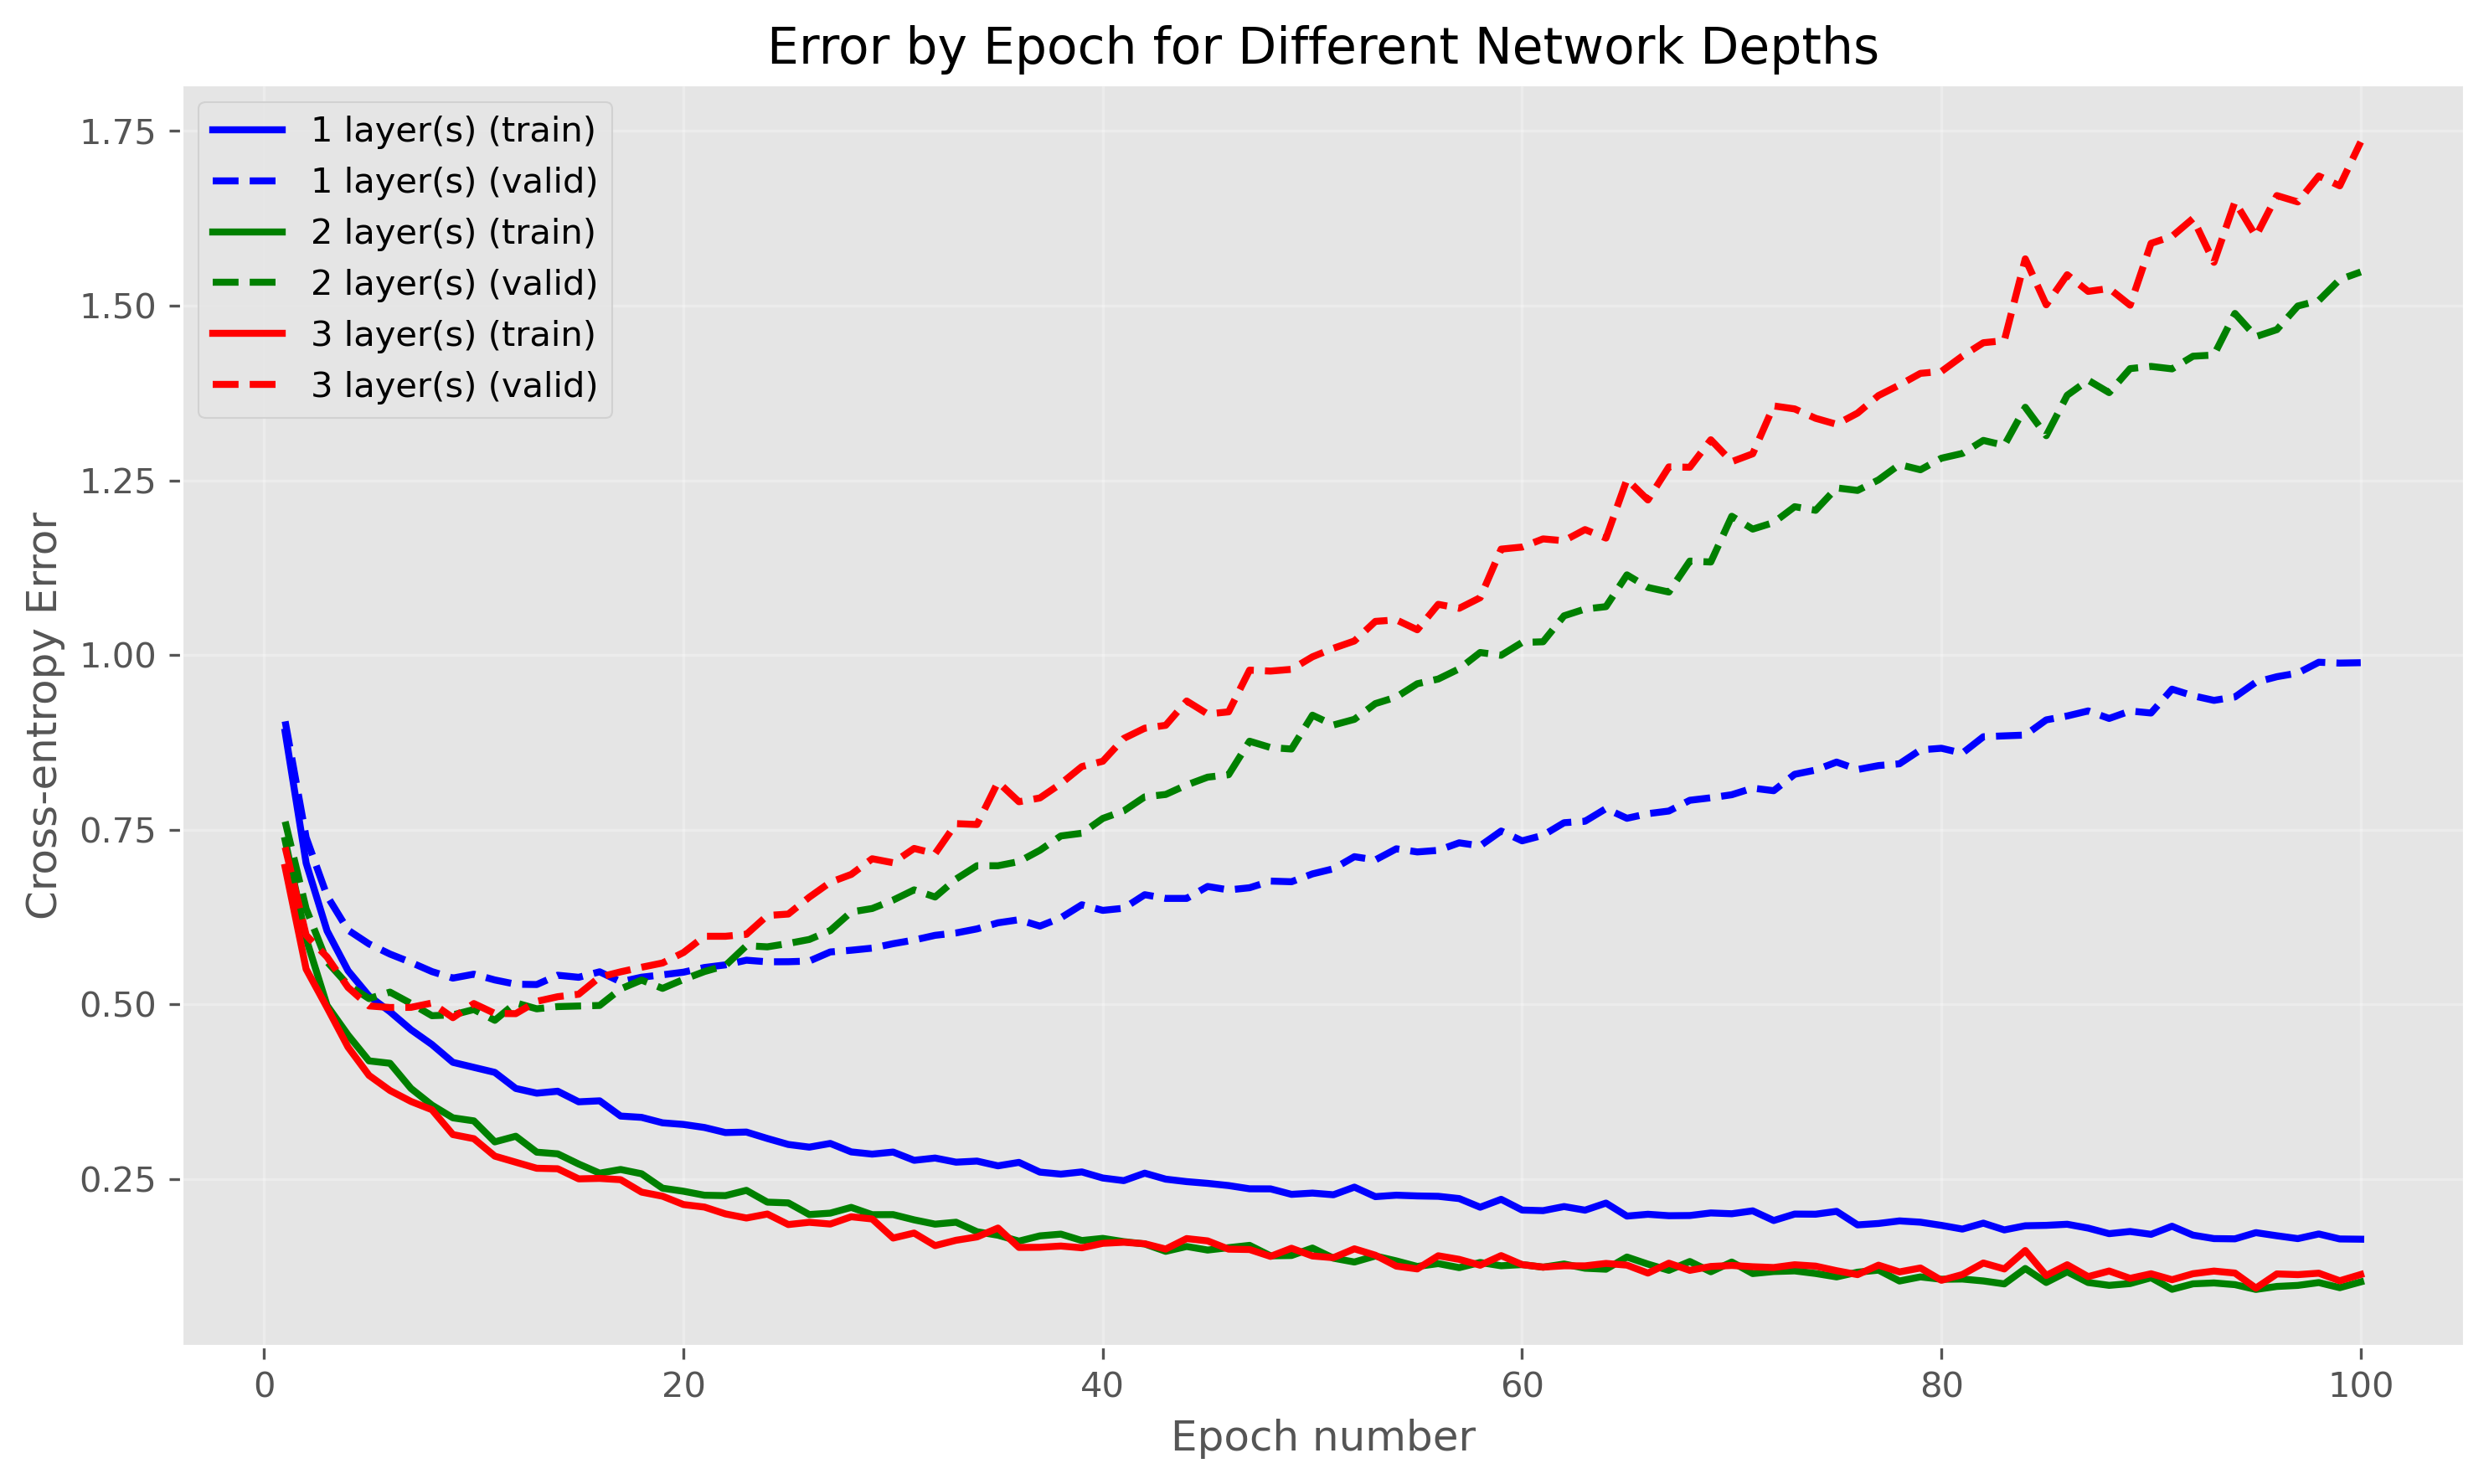
\includegraphics[width=\linewidth]{figures/empty_error_curve_depth.png}
        \caption{error by epoch}
        \label{fig:depth_errorcurves}
    \end{subfigure} 
    \caption{Training and validation curves in terms of classification accuracy (a) and cross-entropy error (b) on the EMNIST dataset for different network depths.}
    \label{fig:depth}
\end{figure} 
}
}

%% Question Figure 4:
\newcommand{\questionFigureFour} {
\youranswer{Question Figure 4 - Replace these images with figures depicting the Validation Accuracy and Generalisation Gap (difference between validation and training error) for each of the experiment results varying the Dropout inclusion rate, and L1/L2 weight penalty depicted in Table 3 (including any results you have filled in).
%
\begin{figure*}[t]
    \centering
    \begin{subfigure}{.475\linewidth}
        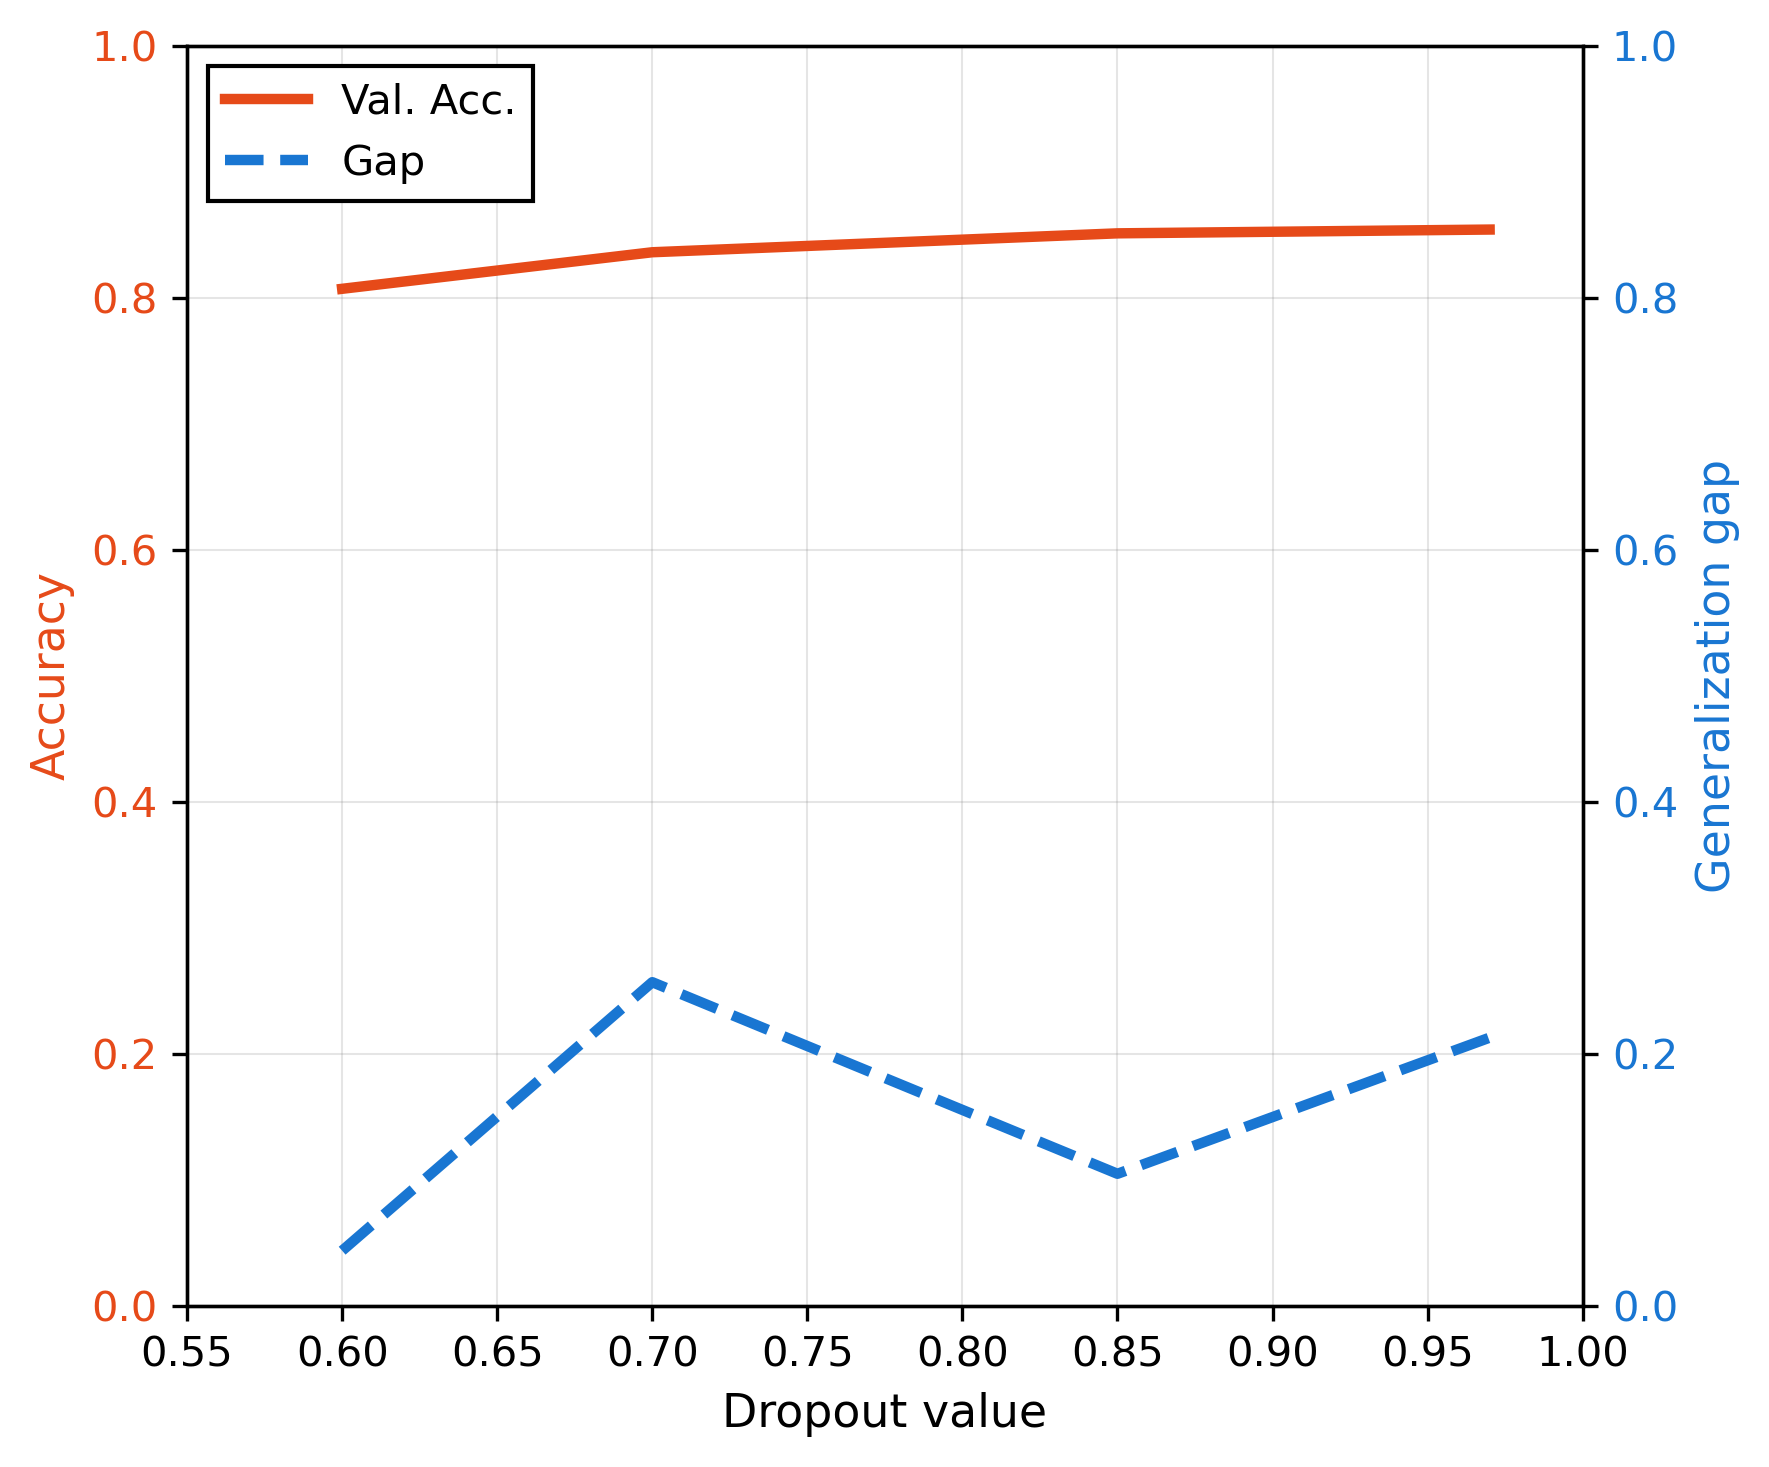
\includegraphics[width=\linewidth]{figures/empty_dropout_plot.png}
        \caption{Accuracy and error by inclusion probability.}
        \label{fig:dropoutrates}
    \end{subfigure} 
    \begin{subfigure}{.475\linewidth}
        \centering
        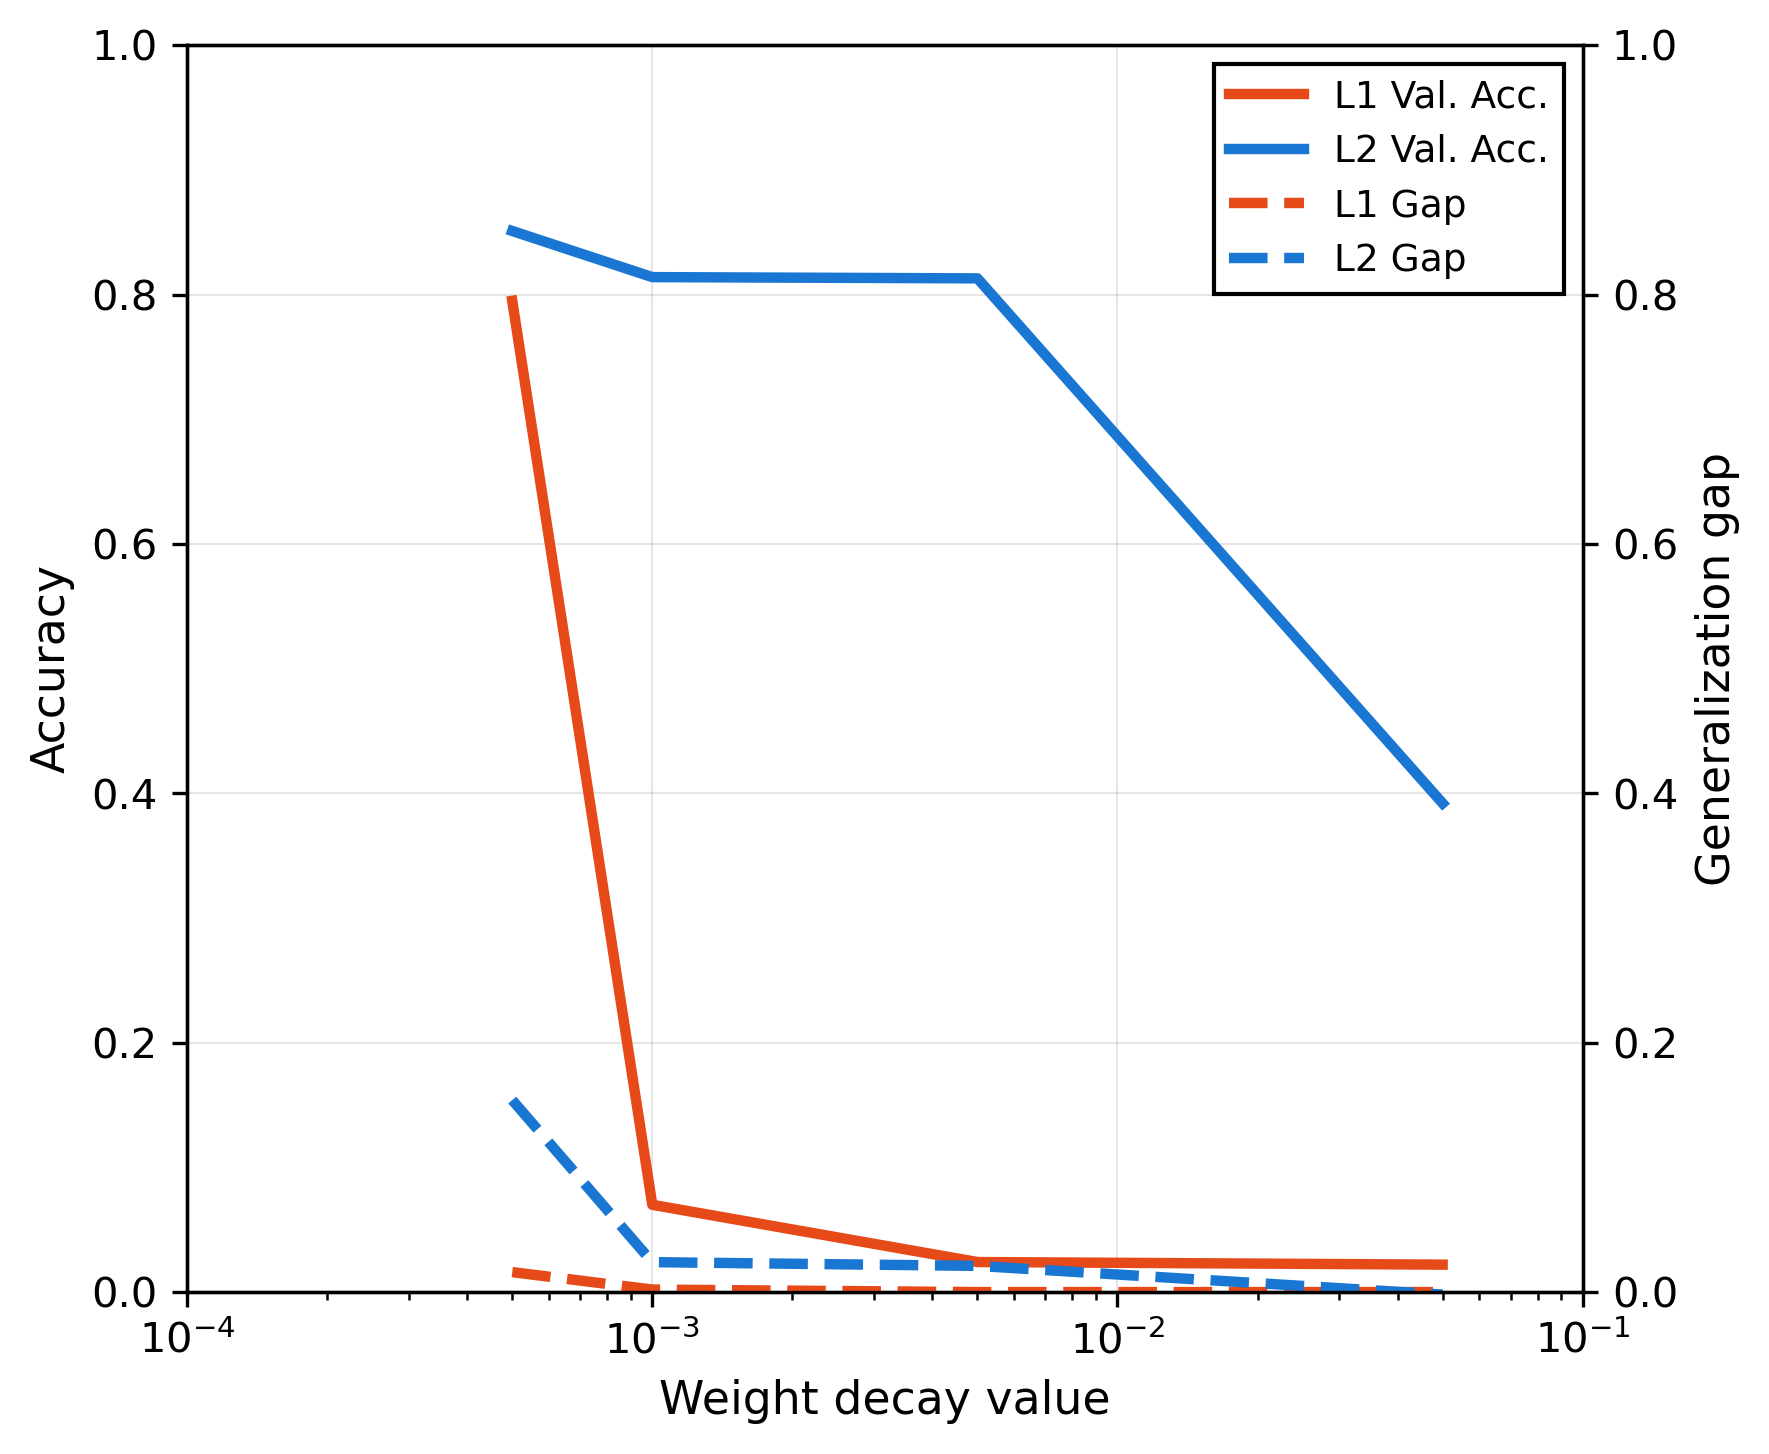
\includegraphics[width=\linewidth]{figures/empty_wd_plot.png}
        \caption{Accuracy and error by weight penalty.}
        \label{fig:weightrates}
    \end{subfigure} 
    \caption{Accuracy and error by regularisation strength of each method (Dropout and L1/L2 Regularisation).}
    \label{fig:hp_search}
\end{figure*}
}
}

%% Question Figure 5:
\newcommand{\questionFigureFive} {
\youranswer{Question Figure 5 - Add figures depicting the Validation Accuracy and Generalisation Gap (difference between validation and training error) for each of your 4 experiments  varying your hyperparameters for the combination of L1 and L2 regularisation (based on your implementation) depicted in Table 4.
}
}

%% Question Figure 6:
\newcommand{\questionFigureSix} {
\youranswer{Question Figure 6 - Add figures depicting the Training Accuracy, Error, and Gradient Flow Across Layers for the 1 experiment run with the Custom Activation function (produce these by running the "Problematic Training" cell in the Coursework\_1.ipynb notebook).
}
}

%% - - - - - - - - - - - - TABLES - - - - - - - - - - - - 

%% Question Table 1:
\newcommand{\questionTableOne} {
\youranswer{
Question Table 1 - Fill in Table 1 with the results from your experiments varying the number of hidden units.
%
\begin{table}[t]
    \centering
    \begin{tabular}{c|ccc}
    \toprule
        \# Hidden Units & Val. Acc. & Train Error & Val. Error\\
    \midrule
        32             &    79.0   &  0.552 &   0.700            \\
        64             &    80.5   &  0.343 &   0.677            \\
        128            &    80.7   &  0.156 &   0.975            \\
    \bottomrule
    \end{tabular}
    \caption{Validation accuracy (\%) and training/validation error (in terms of cross-entropy error) for varying network widths on the EMNIST dataset.}
    \label{tab:width_exp}
\end{table}
}
}

%% Question Table 2:
\newcommand{\questionTableTwo} {
\youranswer{
Question Table 2 - Fill in Table 2 with the results from your experiments varying the number of hidden layers.
%
\begin{table}[t]
    \centering
    \begin{tabular}{c|ccc}
    \toprule
        \# Hidden Layers & Val. Acc. & Train Error & Val. Error \\
    \midrule
        1                 &      80.2      &   0.164 & 0.989                \\
        2                 &      81.6      &   0.103 & 1.548                \\
        3                 &      82.1      &   0.113 & 1.734                \\
    \bottomrule  
    \end{tabular}
    \caption{Validation accuracy (\%) and training/validation error (in terms of cross-entropy error) for varying network depths on the EMNIST dataset.}
    \label{tab:depth_exps}
\end{table}
}
}

%% Question Table 3:
\newcommand{\questionTableThree} {
\youranswer{
Question Table 3 - Fill in Table 3 with the results from your experiments for the missing hyperparameter values for each of L1 regularisation, L2 regularisation, Dropout and label smoothing (use the values shown on the table).
%
\begin{table*}[t]
    \centering
    \begin{tabular}{c|c|ccc}
    \toprule
        Model    &  Hyperparameter value(s) & Validation accuracy & Train Error & Validation Error \\
    \midrule
    \midrule
        Baseline &  -                    &               0.837 &       0.241 &  0.533          \\
    \midrule
        \multirow{4}*{Dropout}
                 & 0.6                   &  80.7                &      0.549 & 0.593     \\
                 & 0.7 & 83.6 & 0.29 & 0.547  \\
                 & 0.85 & 85.1 &  0.329 &  0.434 \\
                 & 0.97 & 85.4 &  0.244 & 0.457  \\
    \midrule
        \multirow{4}*{L1 penalty}
                 & 5e-4 & 79.5 & 0.642 & 0.658 \\
                 & 1e-3 & 7.00 & 1.062 & 1.064 \\
                 & 5e-3 & 2.41 & 3.850 & 3.850 \\
                 & 5e-2 & 2.20 & 3.850 & 3.850 \\
    \midrule
        \multirow{4}*{L2 penalty}  
                 & 5e-4 & 85.1 & 0.306 & 0.460 \\
                 & 1e-3 & 81.4 & 0.600 & 0.624 \\
                 & 5e-3 & 81.3 & 0.586 & 0.607 \\
                 & 5e-2 & 39.2 & 2.258 & 2.256  \\
    \midrule
        Label smoothing & 0.1 & 83.0 & 1.060 & 0.646 \\
    \bottomrule
    \end{tabular}
    \caption{Results of all hyperparameter search experiments. \emph{italics} indicate the best results per series (Dropout, L1 Regularisation, L2 Regularisation, Label smoothing) and \textbf{bold} indicates the best overall.}
    \label{tab:hp_search}
\end{table*}
}
}


%% Question Table 4:
\newcommand{\questionTableFour} {
\youranswer{
Question Table 4 - Add a table with the results from your 4 experiments (by which we mean: 4 training runs, NOT 4 sets of experiments) varying your hyperparameters for the combination of L1 and L2 regularisation (based on your implementation).
%
\begin{table}[!htbp]
    \centering
    \begin{tabular}{l|cc|ccc}
    \toprule
        Configuration & $\lambda_1$ & $\lambda_2$ & Val. Acc. (\%) & Train Error & Val. Error \\
    \midrule
        Conservative       & 0.0005 & 0.0005 & 75.6 & 0.855 & 0.859 \\
        L2-dominant-1      & 0.0001 & 0.0005 & 82.1 & 0.583 & 0.600 \\
        Balanced           & 0.0005 & 0.001 & 73.9 & 0.938 & 0.938 \\
        L2-dominant-2      & 0.0001 & 0.001 & 79.7 & 0.685 & 0.692 \\
    \bottomrule
    \end{tabular}
    \caption{Results of L1+L2 Elastic Net regularization with varying hyperparameters.}
    \label{tab:l1l2_combo}
\end{table}
}
}

%% END of YOUR ANSWERS